% \documentclass[]{amsbook}
\documentclass[]{article}

% \input MyMacros.tex

\usepackage{graphicx}% Include figure files
\usepackage{dcolumn}% Align table columns on decimal point
\usepackage{bm}% bold math
% \usepackage{pictex}%
\usepackage{verbatim} % this is needed for \begin{comment} ... \end{comment}
\usepackage{lscape} % this is needed for occasional landscape figures
\usepackage{amsmath}
% \usepackage{appendix}
% \usepackage{subfigure}
\usepackage{epsfig}
\usepackage{amsfonts}
\usepackage[margin=1.1in, top=1.1in, bottom=1.1in]{geometry}

% \textwidth 550pt
% \textheight 500pt
% \hoffset -3.5cm
\def\betabold{{\pmb{$\beta$}}}

\setcounter{tocdepth}{3}
%
\begin{document}

\date{November 16, 2019}

% \voffset=1.5
\title{
\centerline{}
\centerline{}
\centerline{}
ETEAPOT EDM, Benchmark-III: Updated Results: \\ 
Dispersion, Longitudinal Dynamics and Synchrotron Oscillations \\
}
\author{J. D. Talman and R. M. Talman
}

\maketitle

%
\begin{abstract}
In this chapter ETEAPOT is used to study longitudinal motion in 
the three benchmark lattices documented in previous chapters.
These lattices have field indices $m=-1$, $m\approx0$, and $m=1$.  Most of the results 
this time are presented only for one or the other of the $m=-1,0,1$ cases, since most 
longitudinal quantities are very nearly the same for all three once their 
vertical tunes have all been adjusted to $Q_y$=0.2.

The three benchmark lattices were chosen to be 
especially simple, with optics dominated by the (weak focusing) electric
bend elements. Unfortunately the resulting quite large dispersion 
complicates the longitudinal dynamics.

Evaluations of dispersion, synchroton oscillations, and physical acceptances
are compared with analytical calculations and with calculations using the same
linearized transfer matrix formalism described in the earlier 
benchmark reports\cite{BenchmarkI}\cite{BenchmarkII}.
Agreement is excellent for the lattice dispersion, but ETEAPOT 
finds small-amplitude synchrotron tunes to be 20\% smaller than the analytic
approximation predicts. This may be due to the neglect (in the analytic calculation)
of the quadrupoles used to adjust the tunes to standard values.  It may
also be due to hypersensitivity resulting from the high lattice dispersion.

Accepting the ETEAPOT simulation results as valid, a detailed study of longitudinal
motion is completed. There is excellent agreement with the expectations for $Q_s$ to 
vary proportional to the square root of RF voltage and for the bunch length to vary 
inversely to the square root of RF voltage.
Stability for at least one million turns is demonstrated for 
sufficiently small synchrotron oscillation amplitude; any spurious growth 
in the simulation has a growth lifetime of at least three million turns.
Both qualitatively and quantitatively synchrotron oscillations seem to behave
in electric lattices much the way they do in magnetic lattices.
\end{abstract}
%

% \date{\today}
% \clearpage
% \tableofcontents

\section{Subtle features of longitudinal motion in all-electric rings}
Evolution through thick elements in ETEAPOT (as in TEAPOT) is analytically
exact. In ETEAPOT this includes also spin evolution.
This exact treatment is only possible for certain electric or magnetic 
force fields---uniform magnetic fields for magnets, inverse square law 
(a.k.a. ``Kepler'') for electric fields. In neither case are the as-built,
realistic accelerator force fields nearly this ideally uniform. In ETEAPOT 
(as in TEAPOT) the deviations from ideal are represented by thin
(and hence symplectic) elements. This approach proved valid in TEAPOT,
for both electrons and positrons, for example in calculating dynamic 
apertures of SSC, LHC, CESR, etc. And we regard the approach to be essential
for faithful spin tracking.

The beauty of point sources is that the force fields of point sources
are central. As
a result their 3D orbits are, in fact, restricted to two dimensional
planes. For non-relativistic Kepler planetary orbits the orbits are
perfect ellipses. The protons in proposed EDM storage rings are
sufficiently relativistic that the orbits are not exactly elliptical,
but the deviations from ideal ellipse show up only in ``advances of
perihelion'' of the order of 45 degrees per revolution. Through short
bend elements the orbits look pretty much like ellipses---in fact they
even look pretty much like circles. The exact analytic expressions can
be represented by ``ellipses'' with ``varying constant'' major axis and 
eccentricity. This evolution is well known and is known to be valid
as long as general relativity effects remains negligible.

The orientation of a (relativistic) Kepler orbit can be specified by
the orientation of its major (or minor) axis, and the particle position
can be specified by a very simple analytic formula (first obtained
by Newton) depending only on an angle $\theta-\theta_0$ which is the angle between
the particle angle $\theta$ and the perihelion angle $\theta_0$.
  
The description of accelerator orbits as (relativistic) Kepler orbits
has one inelegant feature; namely, on the central design orbit, the orbit is
circular and there is no unambiguous perihelion angle. In this sense,
\emph{the central orbit is singular}. In principle this
should not be a problem, as the code can define the perihelion angles
arbitrarily for each particle and then keep track of their evolutions.
This includes the requirement, when the orbit switches from oblate 
to prolate, for $\theta_0$ to change discontinuously. 
\emph{This is easier said than done.}

%
\begin{figure}[h]
\centering
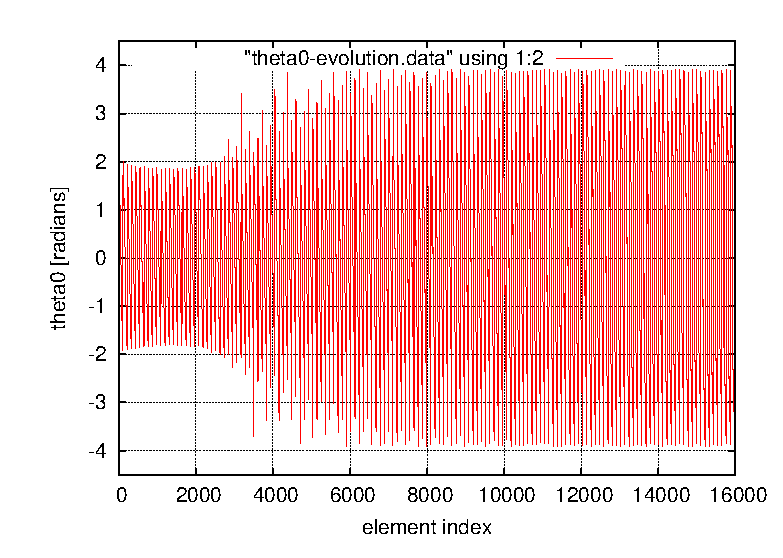
\includegraphics[scale=0.8]{eps/theta0-evolution.eps}
\caption{\label{fig:theta0-evolution}Evolution of perihelion angle $\theta_0$
for 100 turns of a single particle in the {\tt E\_BM\_M1.0.RF} proton EDM ring.
as discussed in the text, erratic behavior starting at element index 3500 or so 
is due to a bug (now removed) in distinguishing between angles of perihelion 
and apheliom.}
\end{figure}
%
Figure~(\ref{fig:theta0-evolution}) shows the evolution
of $\theta_0$ for a particle being tracked through 16,000 elements
(which is about 100 revolutions) around the {\tt E\_BM\_M1.0.RF} ring. 
It can be seen that the evolution of $\theta_0$ is somewhat erratic.
For the first 3000 or so elements $\theta_0$ oscillates between two
extremes. One would prefer a ``constant'' to be more nearly constant than this,
but the behaviour is not unexpected, as the orbit switches periodically from
oblate to prolate (relative to the selected perihelion or aphelion angle).

Because the particle evolution through bend elements depends only
on $\theta-\theta_0$, this alternation has no effect on the calculated
transverse orbit evolution. But the longitudinal effect of the alternation 
was not handled correctly in preliminary ETEAPOT time of flight calculations. 
This bug caused the longitudinal evolution to be treated incorrectly. 

One effect of this error was to destroy reflection symmetry in the horizontal
($ct$-axis) phase space plot). Fixing the bug restored this symmetry. 
(See Figure~\ref{fig:LongitPhSp_BM_M1.0}.) As it happens, the longitudinal 
stability seemed to be not very much disturbed, though fixing the bug altered 
the synchrotron tune by about 30 percent.

There is a further, and more disturbing, feature of Figure~\ref{fig:theta0-evolution}.
It is the erratic variation of $\theta_0$ which is first visible on turn 
3500 or so. Zooming in on this region one sees that, when the orbit
is quite accurately circular, the perihelion can jitter back and forth
several times before settling down to steady alternation.
This seems to have been the source of the (non-Liouvillian) beam growth,
referred to as resonant blow-up in a preliminary report.

As described so far ETEAPOT can be described as ``geometric''. From
an aesthetic point of view this is quite elegant. One sees however, that,
as mentioned above, the fact that the design orbit is singular, essentially
guarantees the existence of occasional jittering between oblate and
prolate parameterizations. Though the code should, in principle, be able
to handle this jittering correctly, the initial code certainly did not. 

The current ETEAPOT code avoids this jittering by introducing a truncated
Taylor series representation of the orbit. This alternate approach is
quite conventional from an accelerator physics standpoint.
Since this code is fully described in the updated {\tt ETEAPOT-expanded.pdf} 
documentation it will not be discussed in detail here. With this code 
incorporated, transverse evolution through bends of every particle is now worked 
out in two different, and almost completely independent, ways.
To avoid the erratic $\theta_0$ determination, only the truncated Taylor series 
approach is used for time of flight calculations. (Technically this requires 
the time of flight to be evaluated using a power series. This is less elegant 
than the analytically exact integral determination, but the series
converges rapidly enough to be essentially exact. This circumvents the 
erratic geometric behavior of near circular orbits.) 

There has been a factor of two computation slow down
resulting from the dual calculations that have been described. We have 
chosen to accept this performance hit for the time being. The performance can be 
recovered either by stripping the code or, better, parallel computation.

The last figure of this section compares transverse evolution
as calculated by the ``geometric'' or ``Mu\~noz'' approach and
by the (more nearly conventional accelerator) truncated Taylor series
approach. 
%
\begin{figure}[h]
\centering
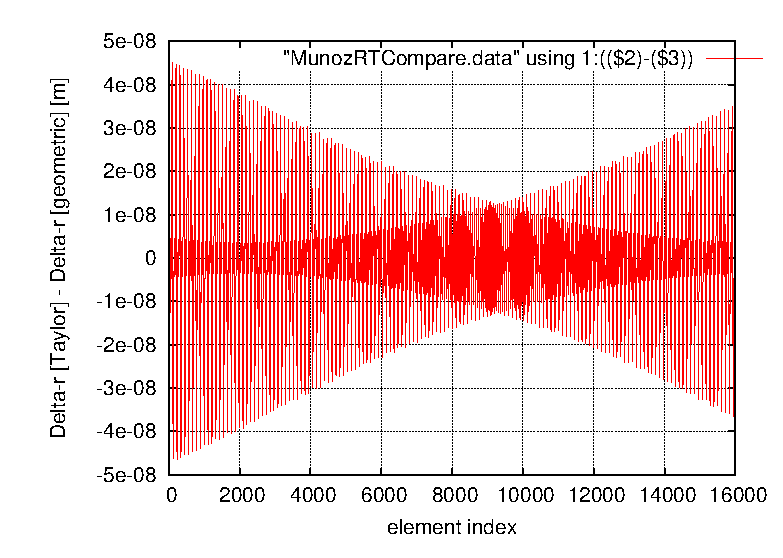
\includegraphics[scale=0.8]{eps/MunozRT-compare.eps}
\caption{\label{fig:MunozRT-compare}Deviation between evolutions of
transverse coordinate $x$ as calculated by (accelerator-style) 
Taylor series formulation and the (geometric, or Mu\~noz, or 
astronomical) formulation.}
\end{figure}
%
Transverse evolution through the same 16,000 elements as
calculated the two independent ways is compared in 
Figure~\ref{fig:MunozRT-compare}. The difference between
radial position calculations never exceeds 
$4.5\times10^{-8}\,$m and, on the average, the deviation
is less than $10^{-9}\,$m. As well as providing
increased confidence in the tracking, this figure also explains
why the (now-repaired) bug affected longitudinal evolution
without affecting transverse evolution.

\section{Parameters of Benchmark Lattices}
Transverse parameters for the benchmark lattices are given in 
Table~\ref{tbl:benchmarkParamsTransv}; these have been copied from
pevious reports. Longitudinal parameters of the same
lattices are given in Table~\ref{tbl:benchmarkParamsLongit}; the
entries are explained in later sections.
%
\begin{table}[h]
\caption{\label{tbl:benchmarkParamsTransv}Transverse parameters of benchmark all-electric 
EDM lattices copied from benchmark comparisons I and II.} 
\medskip
\centering
\begin{tabular}{|c|c|c|c|c|c|c|c|c|}           \hline
file name         & variable name     & unit & {\tt E\_BM\_M1.0.RF.sxf} & {\tt E\_BM\_Z.RF.sxf} & {\tt E\_BM\_P1.0.RF.sxf} \\ 
\hline
cells/arc         & {\tt NCellPerArc} &      &      20               &       20           &        20             \\
bend radius       &  {\tt r0}         &  m   &     40.0              &      40.0          &       40.0            \\
half drift length &  {\tt Ldh}        &  m   &      1.0              &     1.0            &        1.0            \\
half bend per cell & {\tt Thetah}     &  r   &   0.078539816         &  0.078539816       &  0.078539816          \\
half bend length  & {\tt Leh}         &  m   &    3.141592           &  3.141592          &   3.141592            \\
circumference     & {\tt circum}      &  m   &   331.327             &   331.327          &    331.327            \\ 
\hline
inverse focal length &  {\tt q}       & 1/m  &    -0.002019          & -0.00005960        &     0.0019075         \\
field index       &  {\tt m}          &      &     -1.0              &  1.0e-10           &         1.0            \\ 
\hline
horizontal beta  & {\tt betax}        &  m   &    35.9237            &  36.1018           &     36.1910            \\
vertical beta     & {\tt betay}       &  m   &   264.182             &  263.620           &     262.237            \\ 
\hline
horizontal tune  &  {\tt Qx}          &      &     1.4605            &   1.4578           &      1.4588            \\
vertical tune     &  {\tt Qy}         &      &     0.20024           &   0.20004          &     0.20047            \\ 
\hline
\end{tabular}
\end{table}
%
%
\begin{table}[h]
\caption{\label{tbl:benchmarkParamsLongit}Longitudinal parameters (in MAD/UAL units) 
for the {\tt E\_BM\_M1.0.RF.sxf} benchmark all-electric EDM lattice.  
Most of these quantities are very nearly the same for the 
{\tt E\_BM\_Z.RF.sxf} and {\tt E\_BM\_P1.0.RF.sxf}.
This can be seen, for example, in Figure~\ref{fig:LongitPhSp_BMs}.
Uncertainties in the analytic values are discussed in the text.
} 
\medskip
\centering
\begin{tabular}{|c|c|c|c|c|c|c|c|c|c|}           \hline
file name         & symbol                & unit               &         analytic                   &   MAPLE               & ETEAPOT \\ 
\hline
Rev. period       & $T_{\rm rev}(\gamma_0)$ & $\mu$s             &        1.846972                    & 1.846972              & 1.846972  \\      
                  & $dT_{\rm rev}/d\gamma|_{\gamma_0}$  & $\mu$s  &       2.49127                      &                       &            \\
RF frequency      & $f_{\rm RF}$            & MHz               &        0.541426\,$h_{\rm RF}$       &              & 0.541426\,$h_{\rm RF}$ \\  
harmonic number   &  $h_{\rm RF}$           &                   &      100                           &                       &     100      \\
RF peak voltage\S &  $\hat V_{\rm RF}$      & kV                &      1.0                           &                       &     1.0    \\
RF phase lag\P    &  $\phi_{\rm RF}$        & radian            &      0.5                           &                       &    0.5    \\ \hline\hline
dispersion        &  $D_{\rm UAL}$          &   m               & 66.9, Eq.(\ref{eq:Offset.8q})      & $24.8\times2.74=67.9$ &  66.9       \\
slip factor       & $\eta_{\rm RF}$         &                   & $\approx$ -0.92, Eq.(\ref{eq:SlipFac.6})    &                       &                                \\
synch. tune (lo)  & $Q_s(10^{-6})$         &                    & $\approx$ 0.0061, Eq.(\ref{eq:SlipFac.7m})  &                       & 0.0049, Fig.\ref{fig:QsVSsqrtVRF} \\
synch. tune (hi)  & $Q_s(2\times10^{-5})$  &                    &                                    &                      & 0.0048, Fig.\ref{fig:Q_sVsSynchAmplitude}  \\ 
\hline
ang. accept. (short) &                    &                    &                                    &                      & $\pm0.0004$, Fig.\ref{fig:PureBetatron_BM_Z}  \\
ang. accept. (long)  &                    &                    &                                    &                      & $<\pm0.0002$, Fig.\ref{fig:LongTerm_x_M1.0}  \\
\hline
\end{tabular}
\medskip
\qquad \S RF voltage drop in GV,\quad\P RF phase shift in units of $2\pi$
\end{table}
%



\section{Comparison of Fractional Momentum and Energy Offset Parameters}
Different communities prefer different definitions of the fractional
momentum or energy offset.  Wollnik (Section 4.1.1.2) defines the 
``rigidity offset'' $\Delta$ of an off-energy particle by  
%
\begin{equation}
r = r_0(1 + \Delta),
\quad\hbox{or}\quad
\delta_{\rm Wollnik} \equiv \Delta = \frac{r - r_0}{r_0},
\label{eq:Offset.1}
\end{equation}
%
where $r_0$ is the nominal bend radius, and $r$ is the radius of
a concentric circular orbit followed by the off-momentum particle.
This is the fractional offset coordinate applicable to the linearized transfer 
matrix benchmark comparison results in this report.  For ``sector bends'' in 
which all orbits enter and exit more or less normal to the edges of the
bend element there is hardly any need to distinguish between radial
offsets outside and inside bend elements.

ETEAPOT (like MAD) defines a fractional energy offset,
%
\begin{equation}
\delta_{\rm UAL} 
 \equiv 
\frac{{\mathcal E}^O-{\mathcal E_0}^O}{p_0^Oc}.
\label{eq:Offset.2}
\end{equation}
%
The superscript $O$ is attached to ${\mathcal E}^O$ and $p^O$ here to specify 
that these quantities are restricted to regions ``outside'' bend regions;
i.e. where the potential energy vanishes. (For ${\mathcal E}$ this notation
is redundant since ${\mathcal E}$ is preserved except in RF cavities. As it
happens it is also redundant for $p_0$ since, by definition, the potential
energy vanishes everywhere on the design orbit.)
%
\begin{itemize}
\item
It is shown in the ETEAPOT manual that the Wollnik
$\Delta$ parameter is related to the MAD/UAL momentum deviation 
factor $\delta_{\rm UAL}$ by
%
\begin{equation}
\Delta 
 =
\Big(1 + \frac{1}{\gamma_0^2}\Big)\,\frac{1}{\beta_0}\,\delta_{\rm UAL}
\quad
\big(
 = 
2.744\,\delta_{\rm UAL}
\quad\hbox{for\ the\ proton\ EDM\ experiment.} 
\big)
\label{eq:chromatic.6q}
\end{equation}
%
\item
A notation commonly employed in the electron and proton accelerator 
worlds (with jargon ``delta p over p'') is
%
\begin{equation}
\delta_p
 \equiv 
\frac{p^O-p_0}{p_0}.
\label{eq:Offset.4}
\end{equation}
%
(We intentionally refrain from introducing a
momentum-inside variable $\delta_{p^I}$; defined in terms of this variable the
dispersion $D_{\delta_{p^I}}$ would be singular for field index $m=0$.)
Relations among fractional \emph{outside} momentum or energy coordinates,
since they are unaffected by potential energy, can be
obtained using standard (for magnetic lattices) kinematic
formulas, starting from
%
\begin{equation}
{\mathcal{E}}^2 = p^2c^2 + m_p^2c^4.
\label{eq:Offset.9}
\end{equation}
%
For example,
%
\begin{equation}
\frac{dp}{p_0}
 =
\frac{1}{\beta_0}\,
\frac{d\mathcal{E}^O}{p_0c},
\quad\hbox{or}\quad
\delta_p = \frac{1}{\beta_0}\,\delta_{\rm UAL}.
\label{eq:Offset.10}
\end{equation}
%
To obtain $\delta_p$ (also known as ``delta p over p'') from 
$\delta_{\rm UAL}$ one must therefore divide $\delta_{\rm UAL}$ by 0.6.
\item
Should one want the absolute change in $\gamma$ corresponding to $\delta_{\rm UAL}$
one has to multiply $\delta_{\rm UAL}$ by $p_0c/(m_pc^2)=0.7/0.938=0.746$.
This relation can also be expressed as 
$d\gamma=\beta_0\gamma_0\delta_{\rm UAL}$.
\end{itemize}
%

Having established the principle behind the $O$-superscript notation,
from here on quantities without superscripts are to be interpreted
as \emph{outside} quantities. This simplifies the discussion of synchrotron
oscillations where it is assumed that the bend field 
electric potential vanishes throughout RF cavities.

\section{Analytic Estimates of Longitudinal Parameters}
This section discusses the analytical treatment used to estimate
parameters for checking the numerical ETEAPOT results. It is the
only section in which it is necessary to deal with the confusing
subject of kinematic quantities in the interior of bend elements.
The (weak) quadrupoles present in the lattice to trim the tunes are 
neglected for this treatment. This causes an uncontrolled, but 
hopefully small, uncertainty in the comparison values. 

\subsection{Qualitative Discussion of Dispersion}
For circular orbits in an electric bend element 
with radial electric field $-E_0$, the radius of 
the central orbit is given by
%
\begin{equation}
r_0 
 =
\frac{m_pc^2/e}{E_0}\,\gamma_0\beta_0^2.
\label{eq:Offset.5}
\end{equation}
%
For field index $m$ the radius of curvature of an off-momentum
circular orbit is given by
%
\begin{equation}
 r
 = 
r_0\,
\Big(
\frac{\gamma_0^2-1}{\gamma_0}\,
\frac{\gamma^I}{{\gamma^I}^2-1}
\Big)^{1/m},
\label{eq:Offset.6}
\end{equation}
%
where $\gamma_0$ is the value on the central orbit. This relationship
is singular for field index $m=0$ (which is also known as the 
``cylindrical'' case because the electrodes giving this radial
dependence are cylindrical). $m=0$ is
also the unique case in which the dependence of electric potential on
radius $r$ is logarithmic and cannot be expressed by a power law.

For values of $m$ near 1 the orbit velocities of off-energy circular 
orbits within bend elements are approximately independent of $r$.
This causes the time of flight of off-energy
closed orbits through arcs (which are perfect circles) 
to be dominated by the arc length, which
is the bend angle multiplied by $r$. Since the speed depends only
weakly on momentum this is ``above transition'' behavior.
On the other hand, off-energy closed orbit path lengths through drifts 
are independent of $\delta_{\rm UAL}$, which causes time of flight of 
off-energy closed orbits through drifts to be dominated by the 
particle speed; this is ``below transition'' behavior. Assuming
the drift lengths are fairly short, the net behavior is 
``above-transition'' like.

For negative $m$ values the radius of the off-energy closed orbit 
inreases with increasing energy offset. The dispersion $D$ is 
therefore positive for $m<0$; furthermore the magnitude $|D|$ 
\emph{increases} as $m$ approaches zero. 
For positive $m$ values (such as the $m=1$ ``spherical case'')
the radius of off-energy closed orbits decrease with increasing
energy offset. The dispersion $D$ is therefore negative for $m>0$;
but the magnitude $|D|$ again \emph{increases} as $m$ approaches zero. 

Realistic lattices also have quadrupoles which affect the dispersion. 
But, since the quadrupoles are very weak in the three benchmark 
lattices, their influence on lattice dispersion can be expected to
be not very important. (For the minimized-dispersion, strong horizontal
focusing, combined function lattices to be recommended as a 
response to results in the present report,
this will no longer be even approximately valid.)  

Combining all these statements, the dispersion function $D$ has to
have a singularity in the vicinity of $m=0$. It is the longitudinal
dynamics (rather than the transverse) that is sensitive to lattice
dispersion. To make them as simple as possible, the $m$-values of the 
three benchmark lattices were chosen close to zero.  Inadvertently this
choice has caused the longitudinal dynamics of the benchmark lattices
to be hyper-sensitive.

An example of this hypersensitivity comes about in comparing computer
simulation and analytic results. The analytic results depend on the
dispersion. But the dispersion is not used, and is not available, during 
particle tracking. This makes it a priori unkown what RF phase will give 
stable longitudinal motion in simulation. We resolve this ambiguity by 
trying two RF phases differing by $\pi$ and choosing the phase that 
gives stable motion.

Another subtle complication of operation near $m=0$ comes
about because a particle having positive velocity offset outside
bends can have either positive or negative velocity offset inside 
bends, depending on the sign of $m$. This dependence is transparent
to the computer simulation but complicates the analytic calculation
of the ``slip factor'' needed to calculate the synchrotron oscillation 
frequency. 
 
In a truly uniform, weak-focusing, electric
ring the off-momentum closed orbits are true circles
with radius $r$, in which case Eq.~(\ref{eq:Offset.6}) 
provides an analytic formula valid for all amplitudes.
For our purposes this is somewhat academic however, as
explicit quadrupoles make the benchmark lattices 
slightly ``separated-function''. Deflections in the 
quadrupoles cause the off-momentum trajectories to be 
somewhat non-circular in the bends. 

\subsection{Dispersion of the Benchmark Lattices}
Of the benchmark lattices, the closest to the ideal
case is the {\tt E\_BM\_Z.RF} lattice for which the
quadrupoles are very weak. We have found however,
after the quadrupoles have been adjusted to give
identical tunes for the three benchmark cases, that
the longitudinal behaviors of the three lattices are
essentially identical. For example we 
will use Eq.~(\ref{eq:Offset.6}) 
to estimate the dispersion for the {\tt E\_BM\_M1.0} lattice.

In Eq.~(\ref{eq:Offset.6}) the value $m=0$ is singular; this corresponds to
the fact that, for $m=0$, $\gamma^I$ is equal to $\gamma_0$, 
independent of $r$. Exploiting this independence, and neglecting
a small $m$-dependent term that comes from treating the radial
electric field as being independent of $r$, the dependence of
$\gamma$ (which, remember, is $\gamma^O$ by definition) and $r$ is
%
\begin{equation}
\mathcal{E}^O
 =
 m_pc^2\gamma
 \approx 
m_pc^2\gamma_0 + eE_0(r-r_0).
\label{eq:Offset.7}
\end{equation}
%
Differentiating with respect to $r$ gives
%
\begin{equation}
d\mathcal{E}^O = eE_0dr.
\label{eq:Offset.8}
\end{equation}
%
Using Eq.~(\ref{eq:Offset.2}), this can be re-expressed as  
%
\begin{equation}
dr = \frac{p_0c/e}{E_0}\,\delta_{\rm UAL}.
\label{eq:Offset.8p}
\end{equation}
%
The UAL-units dispersion is therefore given by
%
\begin{equation}
r_{\rm co}(\delta_{\rm UAL})
 =
D_{\rm UAL}\delta_{\rm UAL},
\quad\hbox{where}\quad
D_{\rm UAL}
 = 
\frac{p_0c/e}{E_0}
 = 
\frac{0.701}{10.48\times10^{-3}}
 =
66.9\,{\rm m}.
\label{eq:Offset.8q}
\end{equation}
%
Figures~\ref{fig:Dispersion_BM_M1.0} and \ref{fig:Dispersion_BM_M1.0.2}
obtained by UAL/ETEAPOT tracking, agree very well with this
estimate. Especially Figure~\ref{fig:Dispersion_BM_M1.0.2}, for
which horizontal betatron motion has been largely eliminated,
the straight line fit using Eq.~(\ref{eq:Offset.8q}) agrees
perfectly with the tracking results.

\subsection{Slip Factor and Synchrotron Tune}
The revolution period of the central particle is given by
%
\begin{equation}
T_{\rm rev}(\gamma_0)
 =
\frac{2\pi r_0 + D_{\rm tot}}{\beta_0c},
\label{eq:SlipFac.1}
\end{equation}
%
where $D_{\rm tot}=331.3274-2\pi\times40=80.0$\,m is the accumulated 
straight section length. 
Neglecting the effect of the quadrupoles,
for an off-momentum closed orbit, the
revolution period is
%
\begin{equation}
T_{\rm rev}(\gamma)
 =
\frac{2\pi r}{\beta_0c} + \frac{D_{\rm tot}}{\beta^Oc}.
\label{eq:SlipFac.2}
\end{equation}
%
The constancy of $\beta$ within the bend region in the $m=0$ 
case is exploited in the first term, but the actual $\beta^O$
value has to be used in the second term. (Because $D_{\rm tot}$
is so short for the benchmark lattices, this term is small for
the benchmark lattices.  But for long straight sections, as in 
the FNAL option, time of flight through straight regions 
strongly influences the longitudinal motion.)

From $\beta^2=1-1/\gamma^2$ we have, evaluated at $\beta=\beta_0$,
$d\beta=d\gamma/(\beta_0\gamma_0^3)$. Using this in 
Eq.~(\ref{eq:Offset.7}), and applying Eq.~(\ref{eq:Offset.8q}),
the off-momentum, outside, velocity is
%
\begin{equation}
\beta^O
 \approx
\beta_0
\Big(
1 + \frac{1}{\beta^2_0\gamma_0^3}\,
\frac{E_0}{m_pc^2/e}\,
D_{\rm UAL}\delta_{\rm UAL}
\Big)
 =
\beta_0
\Big(
1 + \frac{D_{\rm UAL}\delta_{\rm UAL}}{r_0\gamma_0^2}.
\Big)
\label{eq:SlipFac.3}
\end{equation}
%
Substituting $r-r_0\approx D_{\rm UAL}\delta_{\rm UAL}$ 
also into Eq.~(\ref{eq:SlipFac.2}) yields
%
\begin{equation}
\frac{T_{\rm rev}(\gamma) - T_{\rm rev}(\gamma_0)}{T_{\rm rev}(\gamma_0)}
  =
\frac{1}{\mathcal{C}}\,
\Big(
2\pi
 \mp
\frac{1}{\gamma_0^2}\,\frac{D_{\rm tot}}{r_0}
\Big)
D_{\rm UAL}\delta_{\rm UAL},
\label{eq:SlipFac.4p}
\end{equation}
%
where $\mathcal{C}$ is the circumference of the design orbit. The $\mp$
factor in the second term allows for the fact that $D_{\rm UAL}$
can have either sign, while the phase slip in the straight section
is necessarily negative.
Edwards and Syphers\cite{EdwSyph} define the ``slip factor'' $\eta_{\rm RF}$
by
%
\begin{equation}
\frac{T_{\rm rev}(\gamma+\Delta\gamma)-T_{\rm rev}(\gamma_0)}{T_{\rm rev}(\gamma_0)}
 =
\frac{\eta_{\rm RF}}{\beta_0^2}\,
\frac{\Delta\gamma}{\gamma_0},
\label{eq:SlipFac.5}
\end{equation}
%
and we obtain
%
\begin{equation}
\eta_{\rm RF}
 =
\beta_0\,
\Big(
2\pi
 \mp
\frac{1}{\gamma_0^2}\,\frac{D_{\rm tot}}{r_0}
\Big)\,
\frac{D_{\rm UAL}}{\mathcal{C}}
 =
-0.92.
\label{eq:SlipFac.6}
\end{equation}
%
As mentioned above, the negative sign is accounted for in the
tracking simulation by shifting the RF phase appropriately
to produce stable motion.

Edwards and Syphers give the synchrotron tune in terms of the slip
factor:
%
\begin{equation}
Q_s 
 =
\sqrt{
\frac{1}{2\pi}
\frac{h_{\rm RF}\eta_{\rm RF}\cos(2\pi{\rm lag})}{\beta_0^2\gamma_0}\,
\frac{V_{\rm RF}}{m_pc^2/e}
}
 =
0.0061.
\label{eq:SlipFac.7m}
\end{equation}
%
The $\eta_{\rm RF}\cos(2\pi{\rm lag})$ product needs to be positive for 
the synchrotron oscillations to be stable. The ${\rm lag}$
factor, which establishes the RF phase, is read in from the SXF
lattice description file. (This is discussed further in a 
concluding section.)

\section{Determination of Dispersion Function from Transfer Matrices}
Orbit evolution from the origin at $s=0$ to
a general position $s$ can be expressed by
a transfer matrix ${\bf M}(s,0)$:
%
\begin{equation}
\begin{pmatrix}
x(s) \\ x'(s) \\ \delta
\end{pmatrix}
  =
\begin{pmatrix}
  M_{11}(s,0)  &  M_{12}(s,0)  &   M_{13}(s,0) \\
  M_{21}(s,0)  &  M_{22}(s,0)  &   M_{23}(s,0) \\
   0      &    0     &    1       
\end{pmatrix}\,
\begin{pmatrix}
x(0) \\ x'(0) \\ \delta
\end{pmatrix}.
\label{eq:Dispersion.2p} 
\end{equation}
%
Note that the third component is conserved except at RF cavities.
Also some of th matrix elements depend on the definition of $\delta$.
After associating a transfer matrix to each of the elements in the ring, 
${\bf M}(s,0)$ is found by ``concatenating'' (i.e. multiplying) these
matrices.

For fully-relativistic magnetic lattices the third component $\delta$ is customarily
referred to as $\delta p/p$, and this coordinate
can be identified almost exactly with $\delta\gamma/\gamma$ or with fractional
energy offset (from the design orbit). 
But for an only weakly-relativistic EDM lattice which, furthermore, has
electric bending, it is necessary to be more careful. For now we leave
the definition of $\delta$ open, planning to replace it by one or the
other of the fractional offset coordinates introduced in the previous
section. Of course the dispersion function $D_{\delta}(s)$ becomes definite only 
when $\delta$ is defined unambiguously.
 
The ``off-momentum closed orbit'' $x_{\rm c.o.}(\delta,s)$ is defined
to be the unique orbit which, for longitudinal phase space displacement 
$\delta$, closes on itself after a complete turn around the ring.
The dispersion is then defined, in linearized approximation, by
%
\begin{equation}
x_{\rm c.o.}(\delta,s)
 =
D_{\delta}(s)\,\delta.
\label{eq:Dispersion.1}
\end{equation}
%
Since the transfer matrix includes a description of the 
influence of energy offset, it can also be used
to find the dispersion function $D_{\delta}(s)$. First the
``fixed point'' at the origin, 
$(D_{\delta}(0), D'_{\delta}(0))$ has to be found.
If the lattice
has mirror symmetry, which is true for the benchmark lattices, 
the origin can be chosen on the axis of symmetry, and $D(s)$ is 
also mirror-symmetric; in this case $D'(s)|_{s=0}=0$. 

Evolution once around
the ring, starting from the origin, of an 
off-energy particle on the closed orbit corresponding to 
its energy is described by the ``once-around'' transfer
matrix ${\bf M}$:
%
\begin{equation}
\begin{pmatrix}
D(0)\,\delta \\ 0 \\ \delta
\end{pmatrix}
  =
\begin{pmatrix}
  M_{11}  &  M_{12}  &   M_{13} \\
  M_{21}  &  M_{22}  &   M_{23} \\
   0      &    0     &    1       
\end{pmatrix}\,
\begin{pmatrix}
D(0)\,\delta \\ 0 \\ \delta
\end{pmatrix}.
\label{eq:Dispersion.2} 
\end{equation}
%
This provides two formulas,
%
\begin{equation}
D(0) 
 =
\frac{M_{13}}{1-M_{11}}
 =
-\frac{M_{23}}{M_{21}},
\label{eq:Dispersion.3} 
\end{equation}
%
one of which can be used as a consistency check.
Evolution around the ring of $D(s)$ and $D'(s)$ is then
given by  
%
\begin{equation}
\begin{pmatrix}
D(s) \\ D'(s) \\ 1
\end{pmatrix}
  =
\begin{pmatrix}
  M_{11}(s)  &  M_{12}(s)  &   M_{13}(s) \\
  M_{21}(s)  &  M_{22}(s)  &   M_{23}(s) \\
   0      &    0     &    1       
\end{pmatrix}\,
\begin{pmatrix}
D(0) \\ 0 \\ 1
\end{pmatrix}.
\label{eq:Dispersion.4} 
\end{equation}
%
Spelled out explicitly,
%
\begin{align}
D(s)
 &=
D(0)\,M_{11}(s)
+M_{13}(s),       \notag \\
D'(s)
 &=
D(0)\,M_{21}(s)
+M_{23}(s).
\label{eq:Dispersion.5} 
\end{align}
%
\clearpage

\section{ETEAPOT Longitudinal Dynamics Plots}
Longitudinal dynamics in lattice {\tt BM\_M1.0.RF} (having $m$=-1) is
shown in Figure~\ref{fig:LongitPhSp_BM_M1.0}.
The three
benchmark lattices are compared in the similar plots of
Figure~\ref{fig:LongitPhSp_BM_P1.0}. For this comparison 
only the three innermost amplitudes
are tracked. In these plots three particles start at the origin
traveling in the forward direction, with fractional
energy offsets $\delta_{\rm UAL}=$ 0.000001, 0.000002, 0.000003.
The three plots are essentially identical. We interpret this
to mean that the quadrupoles adjacent to the bend elements,
having been adjusted to restore the vertical tune to its
standard value $Q_y=0.2$, effectively cancel the
focusing effect coming from non-zero field index $m$.
In other words, as far as longitudinal dynamics is concerned,
the three benchmark lattices are equivalent.

Fractional offset 
$\delta_{\rm UAL}\equiv\delta{\mathcal{E}}/(p_0c)$ is
plotted against turn number for a range of 
values of RF amplitude $\hat V_{\rm RF}$ in 
Figure~\ref{fig:delta_vs_turn_V}.  The corresponding longitudinal
phase space plots are shown in Figure~\ref{fig:delta_vs_ct_V}.
%
\begin{figure}[h]
\centering
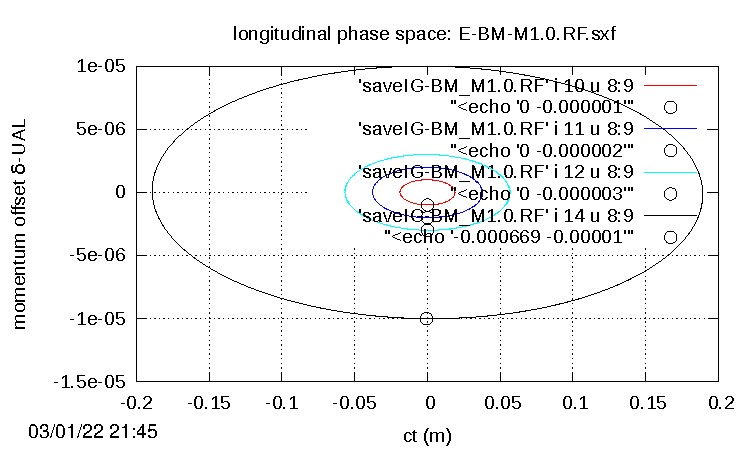
\includegraphics[scale=1.2]{pdf/BM-III_Figure3.pdf}
\caption{\label{fig:LongitPhSp_BM_M1.0}The longitudinal phase space for 
the {\tt BM\_M1.0.RF} lattice is extended to large amplitudes approaching
the limit of stability for the given RF parameters.
Fractional energy offsets are 
$\delta_{\rm UAL}=$ 0.000001, 0.000002, 0.000003, 0.000010. Unlike
the inner three contours, for the outermost contour the particle was 
launched with negligible initial betatron amplitude. 
}
\end{figure}
%

%
\begin{figure}[h]
\begin{minipage}{\linewidth}
\centering
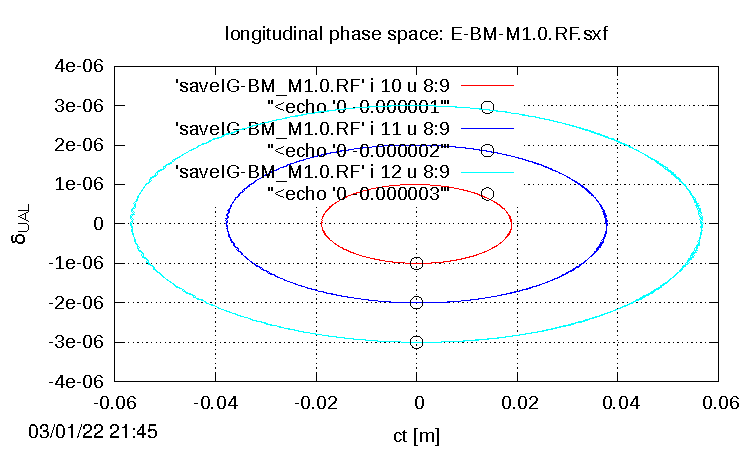
\includegraphics[scale=0.9]{pdf/BM-III_Figure4t.pdf}
\end{minipage}
%
\begin{minipage}{\linewidth}
\centering
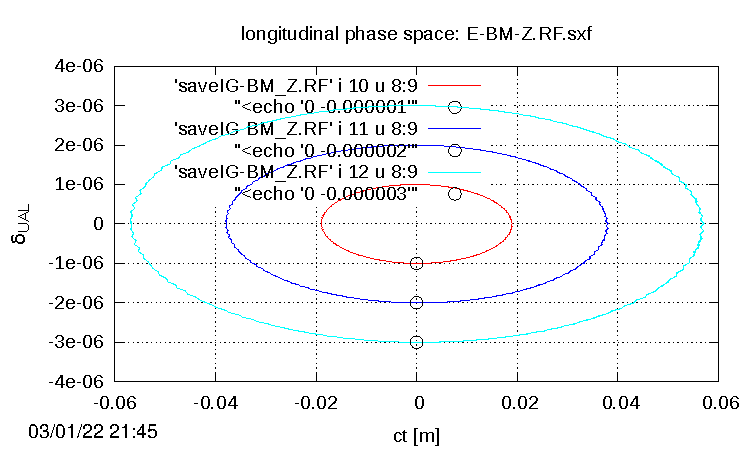
\includegraphics[scale=0.9]{pdf/BM-III_Figure4m.pdf}
\end{minipage}
%
\begin{minipage}{\linewidth}
\centering
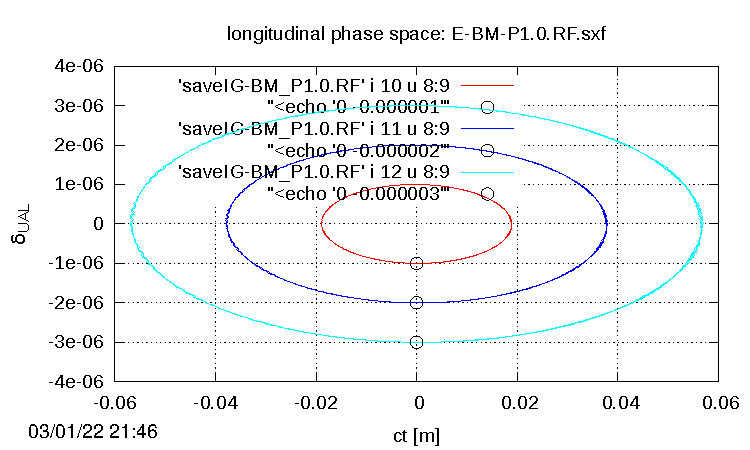
\includegraphics[scale=0.9]{pdf/BM-III_Figure4b.pdf}
\end{minipage}
\caption{\label{fig:LongitPhSp_BMs}
Longitudinal phase space plots for 
lattices (from top to bottom)
{\tt BM\_M1.0.RF}, {\tt BM\_Z.RF}, and {\tt BM\_P1p0.RF}.
}
\end{figure}
%

%
\begin{figure}[h]
\begin{minipage}[b]{0.45\linewidth}
\centering
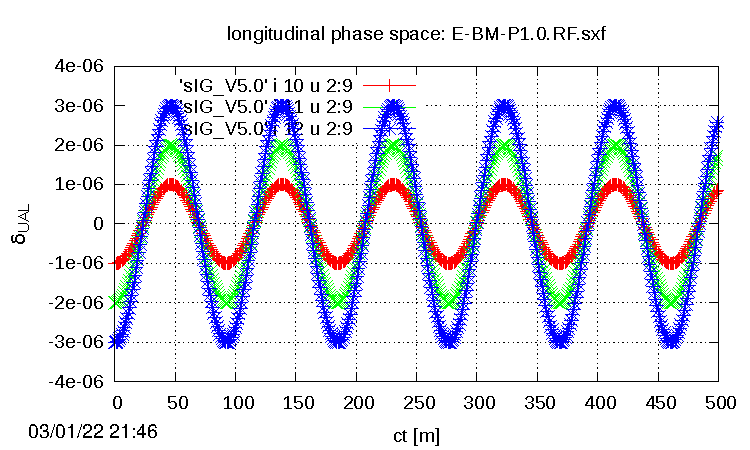
\includegraphics[scale=0.55]{pdf/delta_vs_turn_V5p0.pdf}
\end{minipage}
%
\begin{minipage}[b]{0.45\linewidth}
\centering
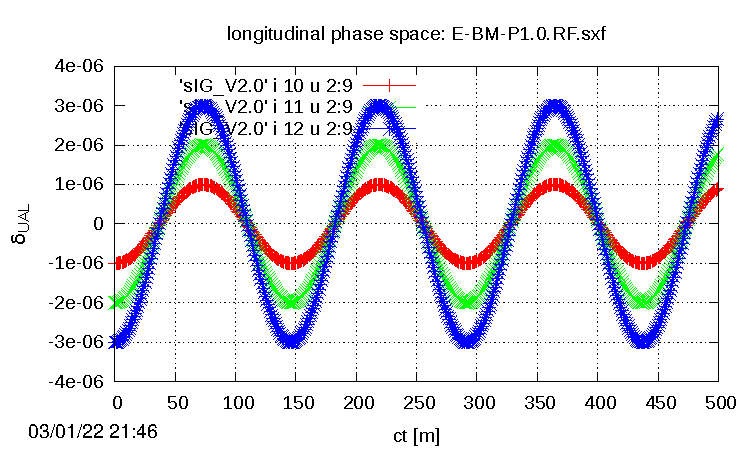
\includegraphics[scale=0.55]{pdf/delta_vs_turn_V2p0.pdf}
\end{minipage}
%
%
\begin{minipage}[b]{0.45\linewidth}
\centering
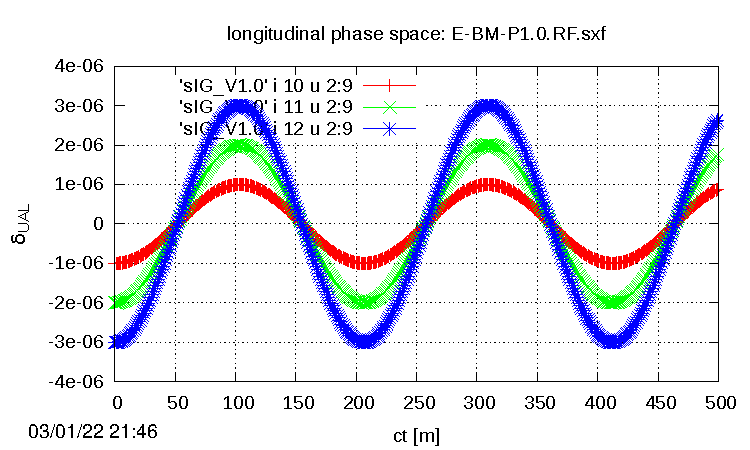
\includegraphics[scale=0.55]{pdf/delta_vs_turn_V1p0.pdf}
\end{minipage}
%
%
\begin{minipage}[b]{0.45\linewidth}
\centering
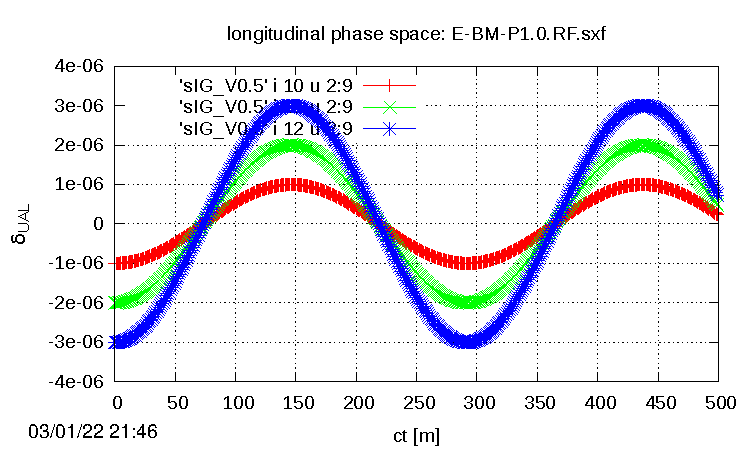
\includegraphics[scale=0.55]{pdf/delta_vs_turn_V0p5.pdf}
\end{minipage}
%
%
\begin{minipage}[b]{0.45\linewidth}
\centering
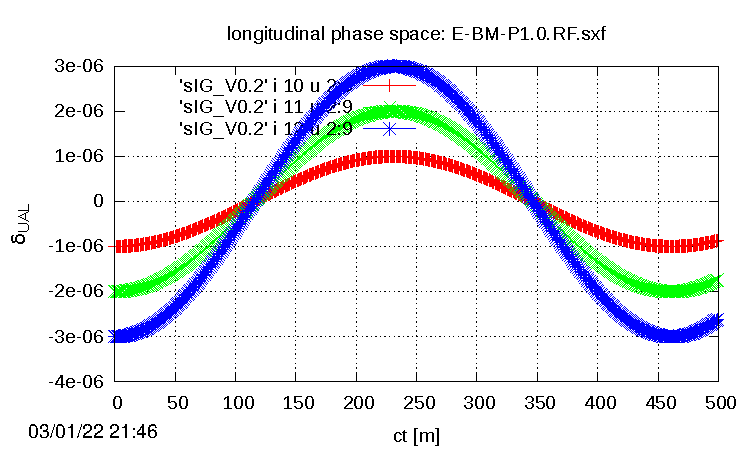
\includegraphics[scale=0.55]{pdf/delta_vs_turn_V0p2.pdf}
\end{minipage}
%
\hskip 1cm
%
\begin{minipage}[b]{0.45\linewidth}
\centering
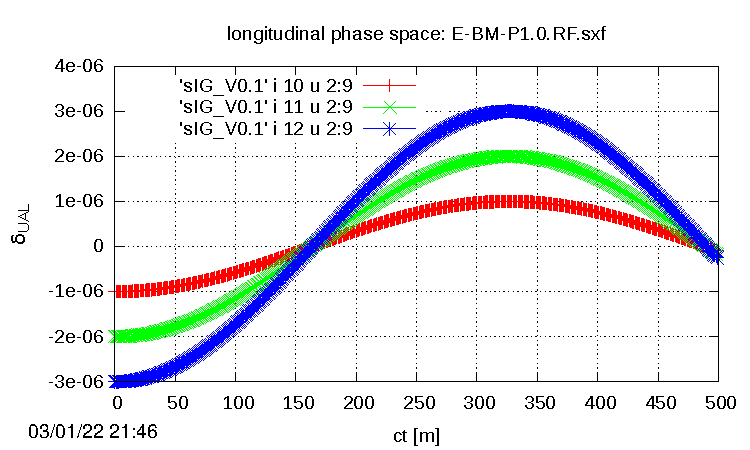
\includegraphics[scale=0.55]{pdf/delta_vs_turn_V0p1.pdf}
\end{minipage}
%
%
\begin{minipage}[b]{0.45\linewidth}
\centering
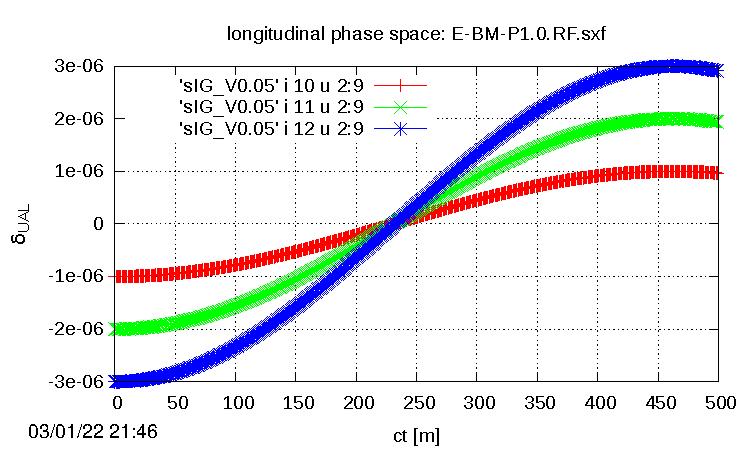
\includegraphics[scale=0.55]{pdf/delta_vs_turn_V0p05.pdf}
\end{minipage}
%
\hskip 1.5cm
%
\begin{minipage}[b]{0.45\linewidth}
\centering
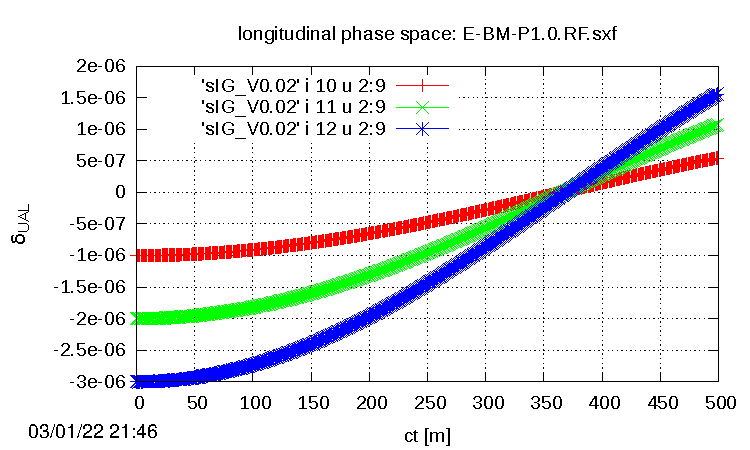
\includegraphics[scale=0.55]{pdf/delta_vs_turn_V0p02.pdf}
\end{minipage}
%
\caption{\label{fig:delta_vs_turn_V}Fractional offset 
$\delta_{\rm UAL}\equiv\delta{\mathcal{E}}/(p_0c)$ 
plotted against turn number for
values of RF amplitude $\hat V_{\rm RF}$
5.0, 2.0, 1.0, 0.5, 0.2, 0.1, 0.05, 0.02 [kV]---reading from
left to right then top to bottom; lattice {\tt BM\_M1.0.RF}.
Each of the plots shows three synchrotron oscillation 
amplitudes. Starting from the origin with vanishing slopes, the
initial ``momentum offsets'' are 
$\delta_{\rm UAL}$=-0.000001,-0.000002, and -0.000003.
}
\end{figure}
%

%
\begin{figure}[h]
\begin{minipage}[b]{0.45\linewidth}
\centering
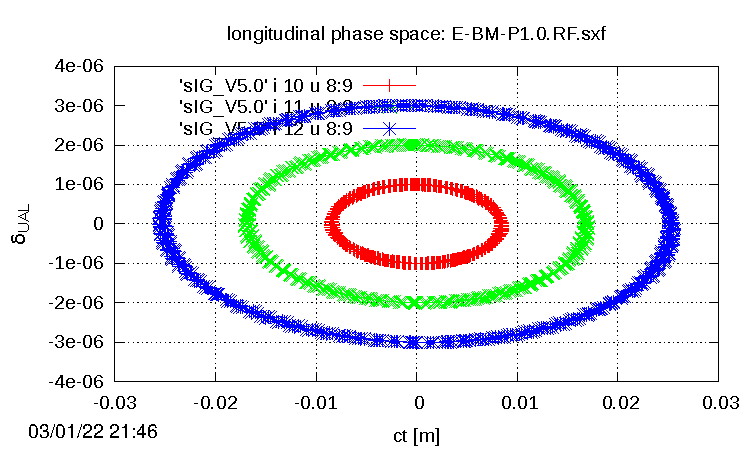
\includegraphics[scale=0.6]{pdf/delta_vs_ct_V5p0.pdf}
\end{minipage}
%
\begin{minipage}[b]{0.45\linewidth}
\centering
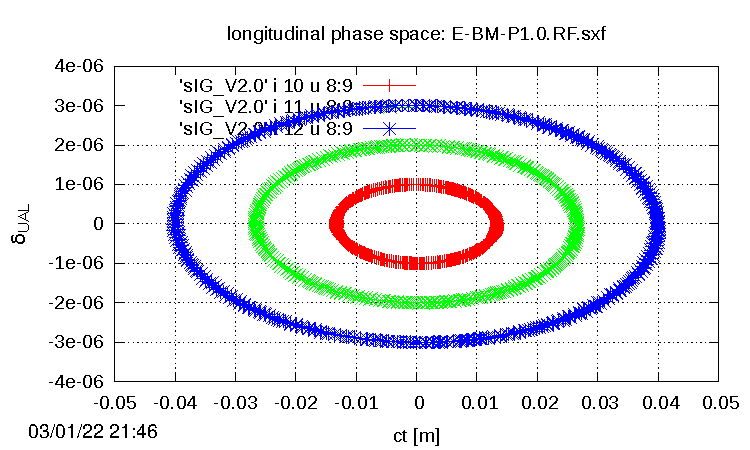
\includegraphics[scale=0.6]{pdf/delta_vs_ct_V2p0.pdf}
\end{minipage}
%
%
\begin{minipage}[b]{0.45\linewidth}
\centering
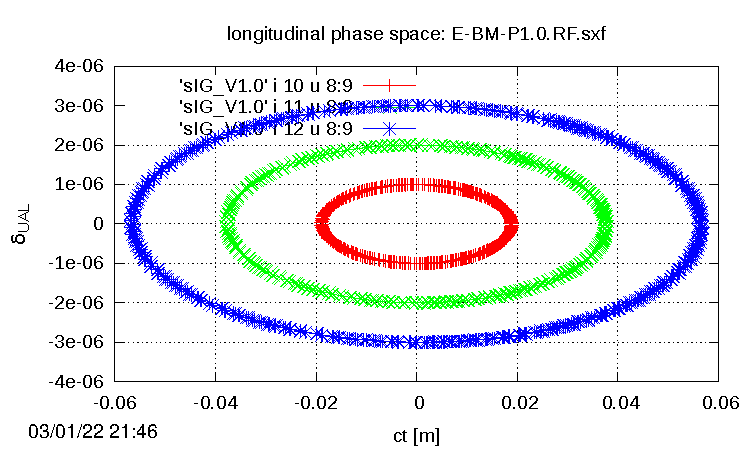
\includegraphics[scale=0.6]{pdf/delta_vs_ct_V1p0.pdf}
\end{minipage}
%
%
\begin{minipage}[b]{0.45\linewidth}
\centering
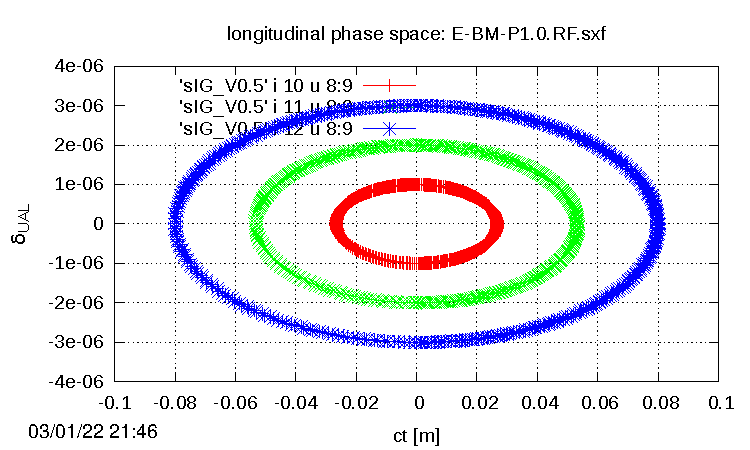
\includegraphics[scale=0.6]{pdf/delta_vs_ct_V0p5.pdf}
\end{minipage}
%
%
\begin{minipage}[b]{0.45\linewidth}
\centering
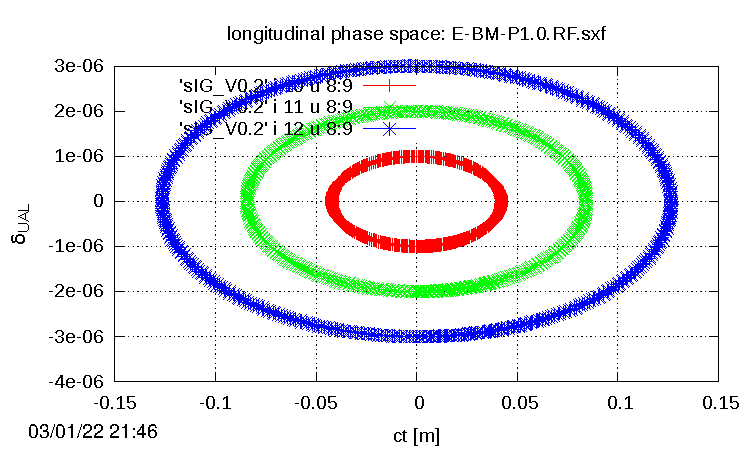
\includegraphics[scale=0.6]{pdf/delta_vs_ct_V0p2.pdf}
\end{minipage}
%
\hskip 1cm
%
\begin{minipage}[b]{0.45\linewidth}
\centering
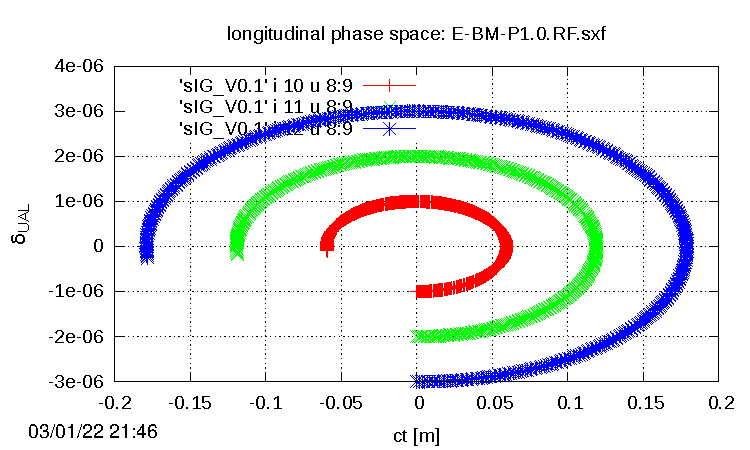
\includegraphics[scale=0.6]{pdf/delta_vs_ct_V0p1.pdf}
\end{minipage}
%
%
\begin{minipage}[b]{0.45\linewidth}
\centering
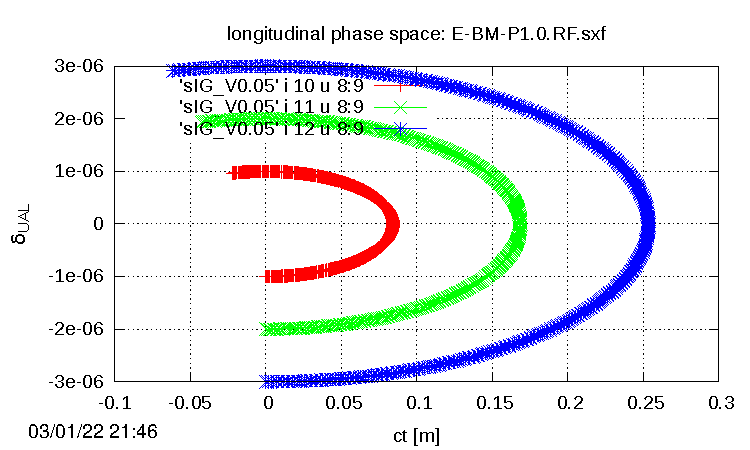
\includegraphics[scale=0.6]{pdf/delta_vs_ct_V0p05.pdf}
\end{minipage}
%
\hskip 1.5cm
%
\begin{minipage}[b]{0.45\linewidth}
\centering
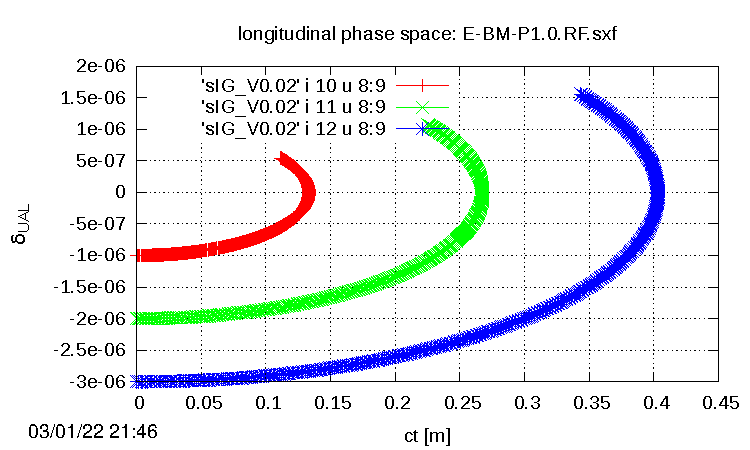
\includegraphics[scale=0.6]{pdf/delta_vs_ct_V0p02.pdf}
\end{minipage}
%
\caption{\label{fig:delta_vs_ct_V}
Longitudinal phase space plots for the same series of RF voltages,
5.0, 2.0, 1.0, 0.5, 0.2, 0.1, 0.05, 0.02\,[kV] as in 
Figure~\ref{fig:delta_vs_turn_V}. The horizontal axis is $z$ in meters.
The vertical axis is the fractional offset 
$\delta{\mathcal{E}}/(p_0c)$.
}
\end{figure}
%

From Figures~\ref{fig:delta_vs_turn_V} and \ref{fig:delta_vs_ct_V}
data can be extracted to produce Figure~\ref{fig:QsVSsqrtVRF} and 
Figure~\ref{fig:BunchlengthVSoneBySqrtVRF} 
which plot the synchrotron tune $Q_s$ and the bunch length $\ell_B$
as functions of $V_{\rm RF}$.
Fitting functions are shown in the
captions to the figures. The strict proportionality 
$Q_s\sim\sqrt{V_{\rm RF}}$ is consistent with Eqs.~(\ref{eq:SlipFac.7m}).  
Also consistent with theory, $\ell_B$ is proportional 
to $1/\sqrt{V_{\rm RF}}$.
%
\begin{figure}[h]
\centering
% \includegraphics[scale=1.0]{Q_sVSsqrtVRF.eps}
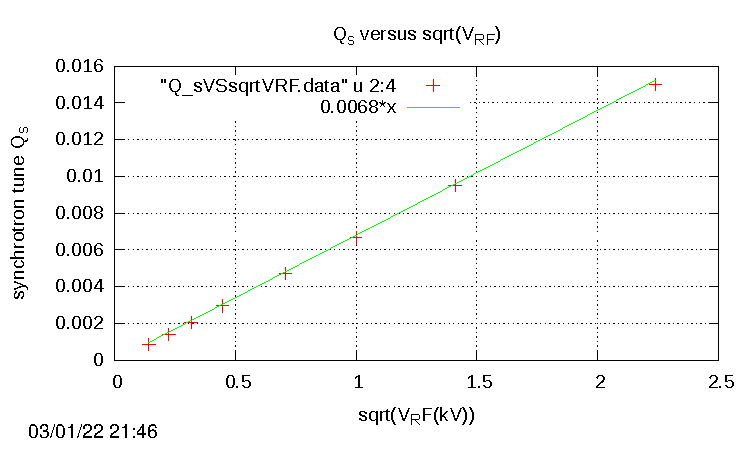
\includegraphics[scale=1.0]{pdf/BM-III_Figure7.pdf}
\caption{\label{fig:QsVSsqrtVRF}Plot of synchrotron tune $Q_s$ 
(obtained by counting periods in plots like those in 
Figure~\ref{fig:delta_vs_turn_V}) versus $\sqrt{V_{\rm RF}[kV]}$.
The fit yields $Q_s=0.00485\sqrt{V_{\rm RF}[kV]}$.
}
\end{figure}
%
%
\begin{figure}[h]
\centering
% \includegraphics[scale=1.0]{BunchlengthVSoneBySqrtVRF.eps}
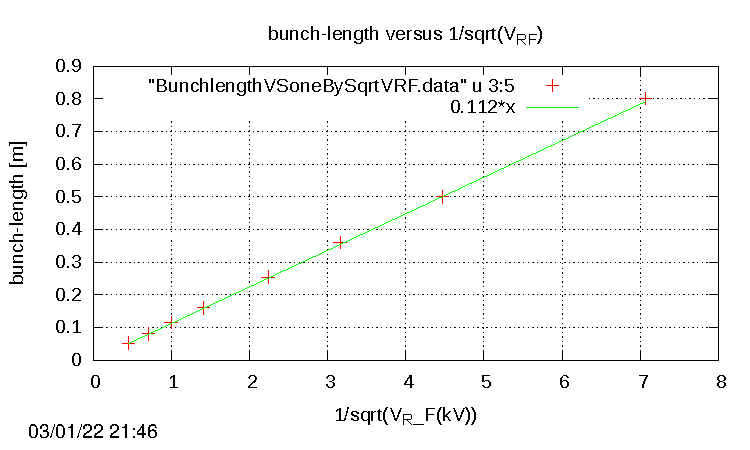
\includegraphics[scale=1.0]{pdf/BM-III_Figure8.pdf}
\caption{\label{fig:BunchlengthVSoneBySqrtVRF}Plot of bunch length
(extremes in plots like those in Figure~\ref{fig:delta_vs_ct_V} for 
$\delta_{\rm UAL}$=0.000003) 
versus $\sqrt{1/V_{\rm RF}[kV]}$.
The fit yields $l_B=0.112\,[{\rm m}]/\sqrt{V_{\rm RF}[{\rm kV}]}$.
}
\end{figure}
%

Another aspect of longitudinal evolution is shown in 
Figure~\ref{fig:Dispersion_BM_M1.0} for 500
turns for the smallest of the three amplitudes
of the run shown in the middle ({\tt E\_BM\_Z.RF.sxf}) case in 
Figure~\ref{fig:LongitPhSp_BM_P1.0}. 
Figure~\ref{fig:Dispersion_BM_M1.0.2} differs only in that initial
conditions have been adjusted to eliminate betatron oscillations.

%
\begin{figure}[h]
\begin{minipage}[b]{\linewidth}
\centering
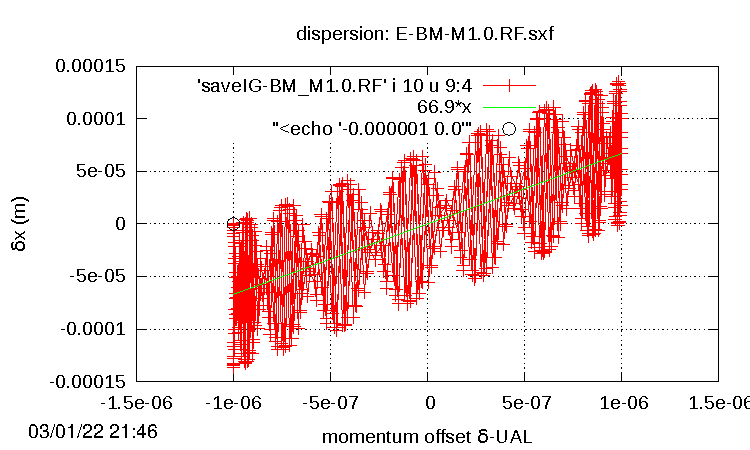
\includegraphics[scale=1.0]{pdf/BM-III_Figure9.pdf}
\caption{\label{fig:Dispersion_BM_M1.0}Starting at the black point, 
radial displacement $x$ is plotted against fractional energy offset 
$\delta_{\rm UAL}$. The straight line corresponding to 
$D_{\rm UAL}=66.9$\,m, as given by Eq.~(\ref{eq:Offset.8q}),
can be seen to give an excellent fit to the data. The scatter of points
can be ascribed to horizontal betatron oscillations.
}
\end{minipage}
\begin{minipage}[b]{\linewidth}
\centering
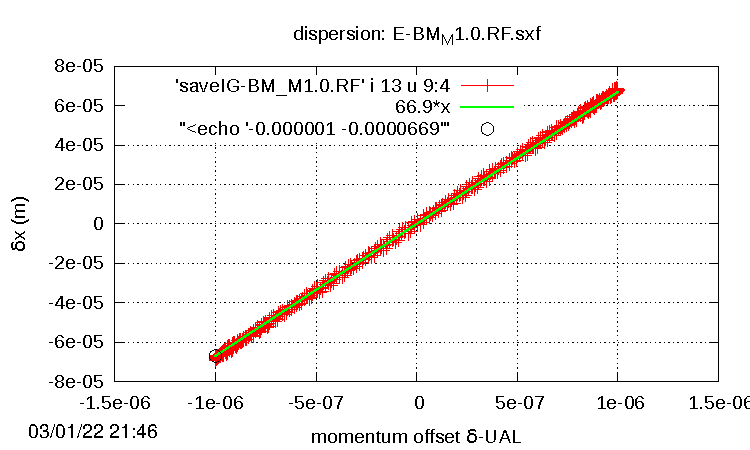
\includegraphics[scale=1.0]{pdf/BM-III_Figure10.pdf}
\caption{\label{fig:Dispersion_BM_M1.0.2}Same as 
Figure~\ref{fig:Dispersion_BM_M1.0} except initial conditions have
been assigned to minimize the initial horizontal betatron oscillation.
So this is pure synchrotron oscillation, with radial
position well fit by $x=66.9[{\rm m}]\delta_{\rm UAL}$.
}
\end{minipage}
\end{figure}
%

In Figure~\ref{fig:PureBetatron_BM_Z} only 
the initial horizontal slope is non-vanishing; $x'=-0.0004$. 
This is approximately the largest angle for which the
particle will not be lost immediately on one of the electrodes
which are situated at $x=\pm0.015\,$m.
The trajectory clearly survives for the interval shown.
Much longer runs will be shown below.

%
\begin{figure}[h]
\begin{minipage}[b]{\linewidth}
\centering
% \includegraphics[scale=0.8]{PureBetatronMinus_BM_M1p0.eps}
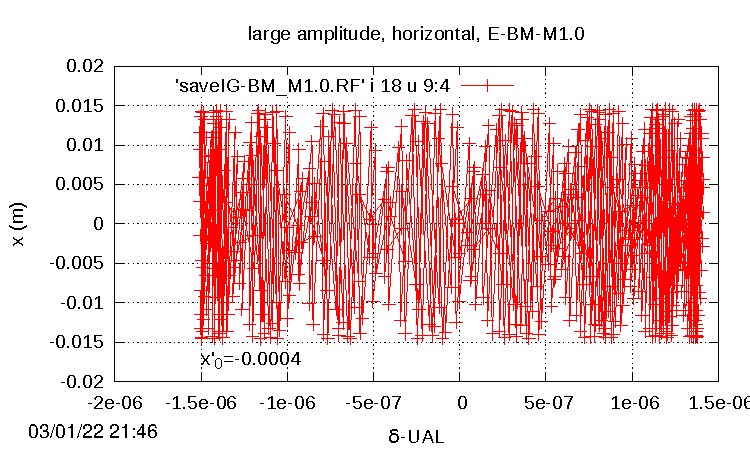
\includegraphics[scale=0.8]{pdf/BM-III_Figure11.pdf}
\end{minipage}
\caption{\label{fig:PureBetatron_BM_Z}Large betatron amplitude,
on-momentum, horizontal betatron motion 
in the {\tt E\_BM\_M1.0.RF.sxf} lattice. 
Initial conditions are $(x=0.0,x'=-0.0004,\delta_{\rm UAL}=0)$.
The graph with opposite initial slope $x'=0.0004$ looks the same.
With gap $g$ being equal to 3\,cm,
this particle is just inside the physical acceptance for
the 500 turns shown.
}
\end{figure}
%

The two graphs of Figure~\ref{fig:Q_sVsSynchAmplitude} 
shows the evolution of longitudinal position $ct$ for small
and large synchrotron oscillation amplitudes. Both
motions are quite accurately sinusoidal.
%
\begin{figure}[h]
\centering
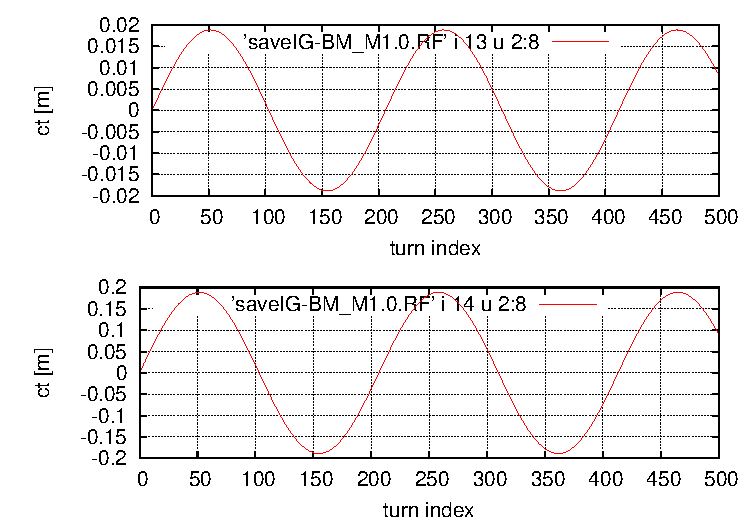
\includegraphics[scale=0.8]{pdf/Q_sVsSynchAmplitude.pdf}
\caption{\label{fig:Q_sVsSynchAmplitude}The upper graph
plots longitudinal position $ct$ vs. turn number for
small amplitude synchroton oscillations. The tune $Q_s$
is $2.45/500=0.0049$. The lower graph
plots the same quantities but for ten times greater
amplitude. The tune $Q_s$ is $2.4/500=0.0048$. 
}
\end{figure}
%

\clearpage

Long term stability is investigated in Figure~\ref{fig:LongTerm_x_M1.0}.
Before the bug fix, for an intermediate case (third from the top), the 
beam blew up radially and fatally after tens of thousands of turns. 
After the bug fix the motion is stable at all investigated amplitudes.

The orbits were stable for one million turns in a weekend long
run. Quantitatively, the exhibited growth, if
interpreted as spurious, would correspond to a spurious growth lifetime
of $3\times10^6$ turns.
%
\begin{figure}[h]
\centering
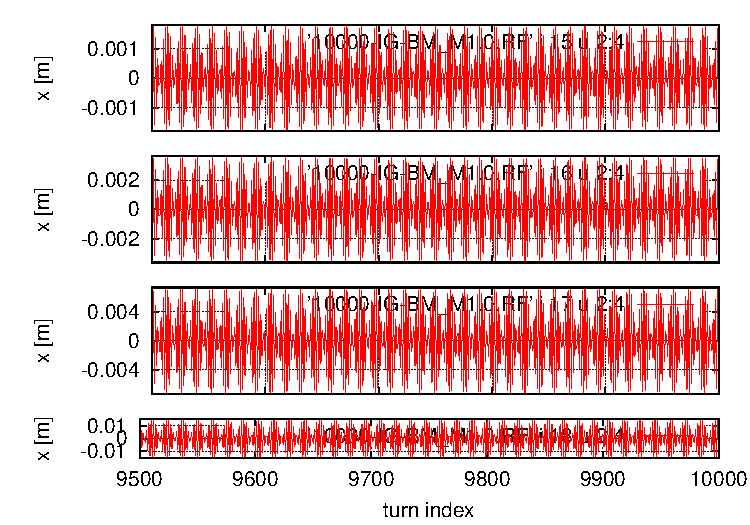
\includegraphics[scale=1.3]{pdf/LongTerm_x_M1p0.pdf}
\caption{\label{fig:LongTerm_x_M1.0}Tracking on-momentum particles
with initial $x'$ slopes of $-0.00005$, $-0.0001$, $-0.0002$,  
and $-0.0004$ for 10,000 turns in the {\tt E\_BM\_M1.0.RF.sxf} 
lattice. Only the last 500 turns are shown. Even the largest
amplitude case is stable indefinitely.
}
\end{figure}
%

\section{Summary}
\subsection{Comments and (Tentative) Conclusions}
With a few significant exceptions, the various plots exhibit 
behaviour much like what one sees in magnetic lattices.
Various numerical comparisons of momentum-dependent ETEAPOT tracking 
results with analytic calculations and with results from the linearized 
transfer matrix model are listed in Table~\ref{tbl:benchmarkParamsLongit}.
We consider the following points to be significant:
%
\begin{itemize}
\item
We have found no significant differences in longitudinal dynamics
among the three benchmark lattices (which have field index $m=-1,0,1$.)
The discrete quadrupoles have been adjusted to give exactly the
same vertical tunes and very nearly the same horizontal tunes. Apparently
this constrains the longitudinal dynamics to be equivalent.
\item
There is essentially perfect agreement on the dispersion
which is $D_{\rm UAL}=66.9\,$m. ($D_{dp/p}=\beta_0D_{\rm UAL}=40.1\,$m.)
Note, for example, Figure~\ref{fig:Dispersion_BM_M1.0.2}, which shows 
pure synchrotron oscillation with $x[m]=66.9\,\delta_{\rm UAL}$.
\item
ETEAPOT's determination of the small amplitude synchrotron tune 
is $Q_s=0.0049$, which is significantly different from the ``analytic''
value $Q_s=0.0061$. Noting that ``analytic'' and ``correct'' are not synonyms, 
clearly one or the other is wrong. Copied from the magnetic
ring formalism, the analytic calculation assumes the absence of coupling
between synchrotron an betatron oscillation, which is patently wrong.
In other words, the analytic result is over-simplified. (The linearized
transfer matrix model determination does not provide an independent 
check of longitudinal motion other than the value of lattice dispersion.)
\item
What makes the determination of synchrotron tune $Q_s$ challenging is that 
it is hard to calculate
the time of flight accurately.  Apart from the fact that the fractional
path length variations are miniscule, the change of velocity caused by
change of potential has to be accounted for very accurately. Our
calculation, based on analytic evaluation of the time of flight
integral should,
however be accurate and has been checked independently. 
We are now evaluating times of flight by two independent methods.
Spot check comparisons of the two methods agree, typically to
eight significant figures. (As it happens, before the bug fix, the 
error in the time of flight calculation was due to error in 
start and stop times rather than incorrect evaluation of the
time of flight integral.)
\item
The ETEAPOT evaluation of spin precession in bend elements proceeds
using formalism just like the time of flight formalism. The
spin precession integrals are elementary and do not require either 
approximate or power series evaluation to be expressable in 
exact closed form.  
\item
The phase space has not been adequately investigated to obtain
an accurate horizontal admittance value. A rough estimate 
derived from just the angular acceptance comes from
$|x'_{\rm max}|\approx\sqrt{\epsilon_{\rm admittance}/\beta_x}$ or 
%
\begin{equation}
\epsilon_{\rm admittance}
\approx
\beta_x{x'_{\rm max}}^2
 =
36\times0.0004^2
 =
5.8\times10^{-6}\,{\rm m}.
\label{eq:Comments.1} 
\end{equation}
%
This is substantially larger than the value $10^{-6}\,${\rm m} used
in some preliminary parameter estimations.
\item
The results of the previous version of this report strongly 
suggested that the magnitude of the lattice dispersion in the 
pEDM benchmark lattices being considered was unacceptably large. 
This may still be true, but that conclusion can no longer
be based on the ETEAPOT tracking, as it was, for example, in 
our separate report\cite{RTMinimumDispersion}.
\item
That report proposed a minimized-dispersion, combined function 
lattice that is strong-focusing horizontally and
(as favored for the EDM measurement) weak-focusing vertically.
Of all the lattices that have been contemplated for the proton
EDM experiment, that alternating gradient lattice most nearly 
resembled the very first all-electric lattice, which was built at 
BNL for the very first alternating gradient proton 
accelerator\cite{Plotkin}.
\item
In that report, both the experience with ELISA and the discouraging
ETEAPOT tracking argued that the EDM ring dispersion had to be 
reduced. The ELISA experience constinues to be worrisome, but the 
(quite limited) ETEAPOT tracking only supports what has
always been known---the injected momentum spread has to be very
small. But long spin coherence time also requires tiny momentum
spread, so these two requirements are, at least, compatible. 
\item
We have therefore reverted to the opinion that it is an open question 
as to whether or not alternating gradient focusing is really 
needed for the proton EDM experiment.
\end{itemize}
%

%
\begin{thebibliography}{99}
\bibitem{BenchmarkI}
J.D. Talman and R.M. Talman, \emph{ UAL/ETEAPOT Results 
(Augmented) for Proton EDM Benchmark Lattices,} BNL internal
report, April 29, 2012

\bibitem{BenchmarkII}
J.D. Talman and R.M. Talman, \emph{ UAL/ETEAPOT Proton EDM 
Benchmark Comparisons II: Transfer Matrices and Twiss Functions,} 
BNL internal report, August 30, 2012

\bibitem{EdwSyph}
D. Edwards and M. Syphers, \emph{Longitudinal Motion,}
p. 53 in \emph{Handbook of Accelerator Physics and Engineering,}
editors, A. Chao and M. Tigner, World Scientific, 2002

\bibitem{ETEAPOT-expanded}
N. Malitsky, J. Talman, and R. Talman, \emph{Appendix UALcode: Development of the
UAL/ETEAPOT Code for the Proton EDM Experiment,} UAL/ETEAPOT documentation
(frequently revised), August, 2012

\bibitem{pEDM}
Storage Ring EDM Collaboration, \emph{A Proposal to Measure the
Proton Electric Dipole Moment with $10^{-29}\,$e-cm Sensitivity,}
especially Appendix 1. October, 2011

\bibitem{RTMinimumDispersion}
R. Talman, \emph{Reduced Dispersion Proton EDM Storage Ring Lattices,}
Internal Report, 12 December, 2012

\bibitem{Plotkin}
M. Plotkin, \emph{The Brookhaven Electron Analog, 1953-1957,} 
Brookhaven Internal Report, BNL-45058, 1991

\bibitem{EtienneBook}
E. Forest, \emph{Beam Dynamics, A New Attitude and Framework,} 
Harwood Academic Publishers, 1998. See especially 
Section 12.2.3,

\end{thebibliography}

\end{document}





\bibitem{Moller}
C. M\o ller, \emph{The Theory of Relativity,} Clarendon Press,
Oxford, 1952, 

\bibitem{Munoz}
G. Mu\~{n}oz and I. Pavic, \emph{A Hamilton-like vector for
the special-relativistic Coulomb problem,} 
Eur. J. Phys. {\bf 27}, 1007-1018, 2006

\bibitem{Talman}
R. Talman, \emph{Geometric Mechanics,} John Wiley and Sons, 2000

\bibitem{Aguirregabiria}
J. Aguirregabiria et al., 
Archiv:physics/0407049v1 [physics.ed-ph] 2004, 

\bibitem{Torkelsson}
U. Torkelsson, Eur. J. Phys., {\bf 19}, 459, 1998, 

\bibitem{Boyer}
T. Boyer, Am. J. Phys. {\bf 72} (8) 992, 2004

